\chapter{Application of Machine Learning Algorithms}
\label{chap:four}

\section{Repository and Environment Structure}
\section{Data Exploration}
This section is focused on exploration of the analyzed loan dataset, particularly on dataset description, distribution analysis and association analysis, in order to infer potential valuable insights and hypotheses which can be used in the preprocessing or modelling part.

\subsection{Dataset Description}
The analyzed dataset pertains to the HMEQ dataset which contains loan application information and default status of 5,960 US home equity loans. Such dataset was acquired from Credit Risk Analytics.

As can be seen, the dataset contains 12 columns, 11 features and 1 target variable \texttt{BAD} indicating whether the loan was in default (\texttt{1}) or not (\texttt{0}). 
Amongst the 11 features, there are 9 numeric features and 2 categorical features, namely \texttt{REASON} which contains 2 categories - Debt consolidation (\texttt{DebtCon}) and Home improvement (\texttt{HomeImp}), and \texttt{JOB} which fontains following categories - Administration (\texttt{Offce}), Sales, Manager (\texttt{Mgr}), Professional Executive (\texttt{ProfExe}), Self-employed (\texttt{Self}), and Other.


\begin{table}[H]
    \small
    \setlength{\tabcolsep}{8pt}
    \renewcommand{\arraystretch}{1.3}
    \begin{center}
        \caption[Dataset columns]{Dataset columns}\label{tab:values}
    \begin{tabular}{@{} l p{8cm} l @{}}
    \toprule
    \textbf{Columns} & \textbf{Description} & \textbf{Data type}\\
    \midrule
    BAD & Default status & Boolean \\
    \hline
    LOAN & Requested loan amount & numeric \\
    \hline
    MORTDUE & Loan amount due on existing mortgage & numeric \\
    \hline
    VALUE & Value of current underlying collateral property & numeric \\
    \hline
    REASON & Reason of loan application & categorical \\
    \hline
    JOB & Job occupancy category & categorical \\
    \hline
    YOJ & Years of employment at present job & numeric \\
    \hline
    DEROG & Number of derogatory public reports & numeric \\
    \hline
    DELINQ & Number of delinquent credit lines & numeric \\
    \hline
    CLAGE & Age of the oldest credit line in months & numeric \\
    \hline
    NINQ & Number of recent credit inquiries & numeric \\
    \hline
    CLNO & Number of credit lines & numeric \\
    \hline
    DEBTINC & Debt-to-income ratio & numeric \\
    \bottomrule
    \end{tabular}
    \end{center}
    \begin{center} % Center the source
    \source{\url{http://www.creditriskanalytics.net/datasets-private2.html}}
    \end{center}
\end{table}


\subsection{Distribution Analysis}
In this subsection, we inspect the distribution of our variables, including the target variable and the features.

Default distribution:

\begin{figure}[H]
    \begin{center}
    \caption{Default status distribution}
    \label{fig:defaultdist}
    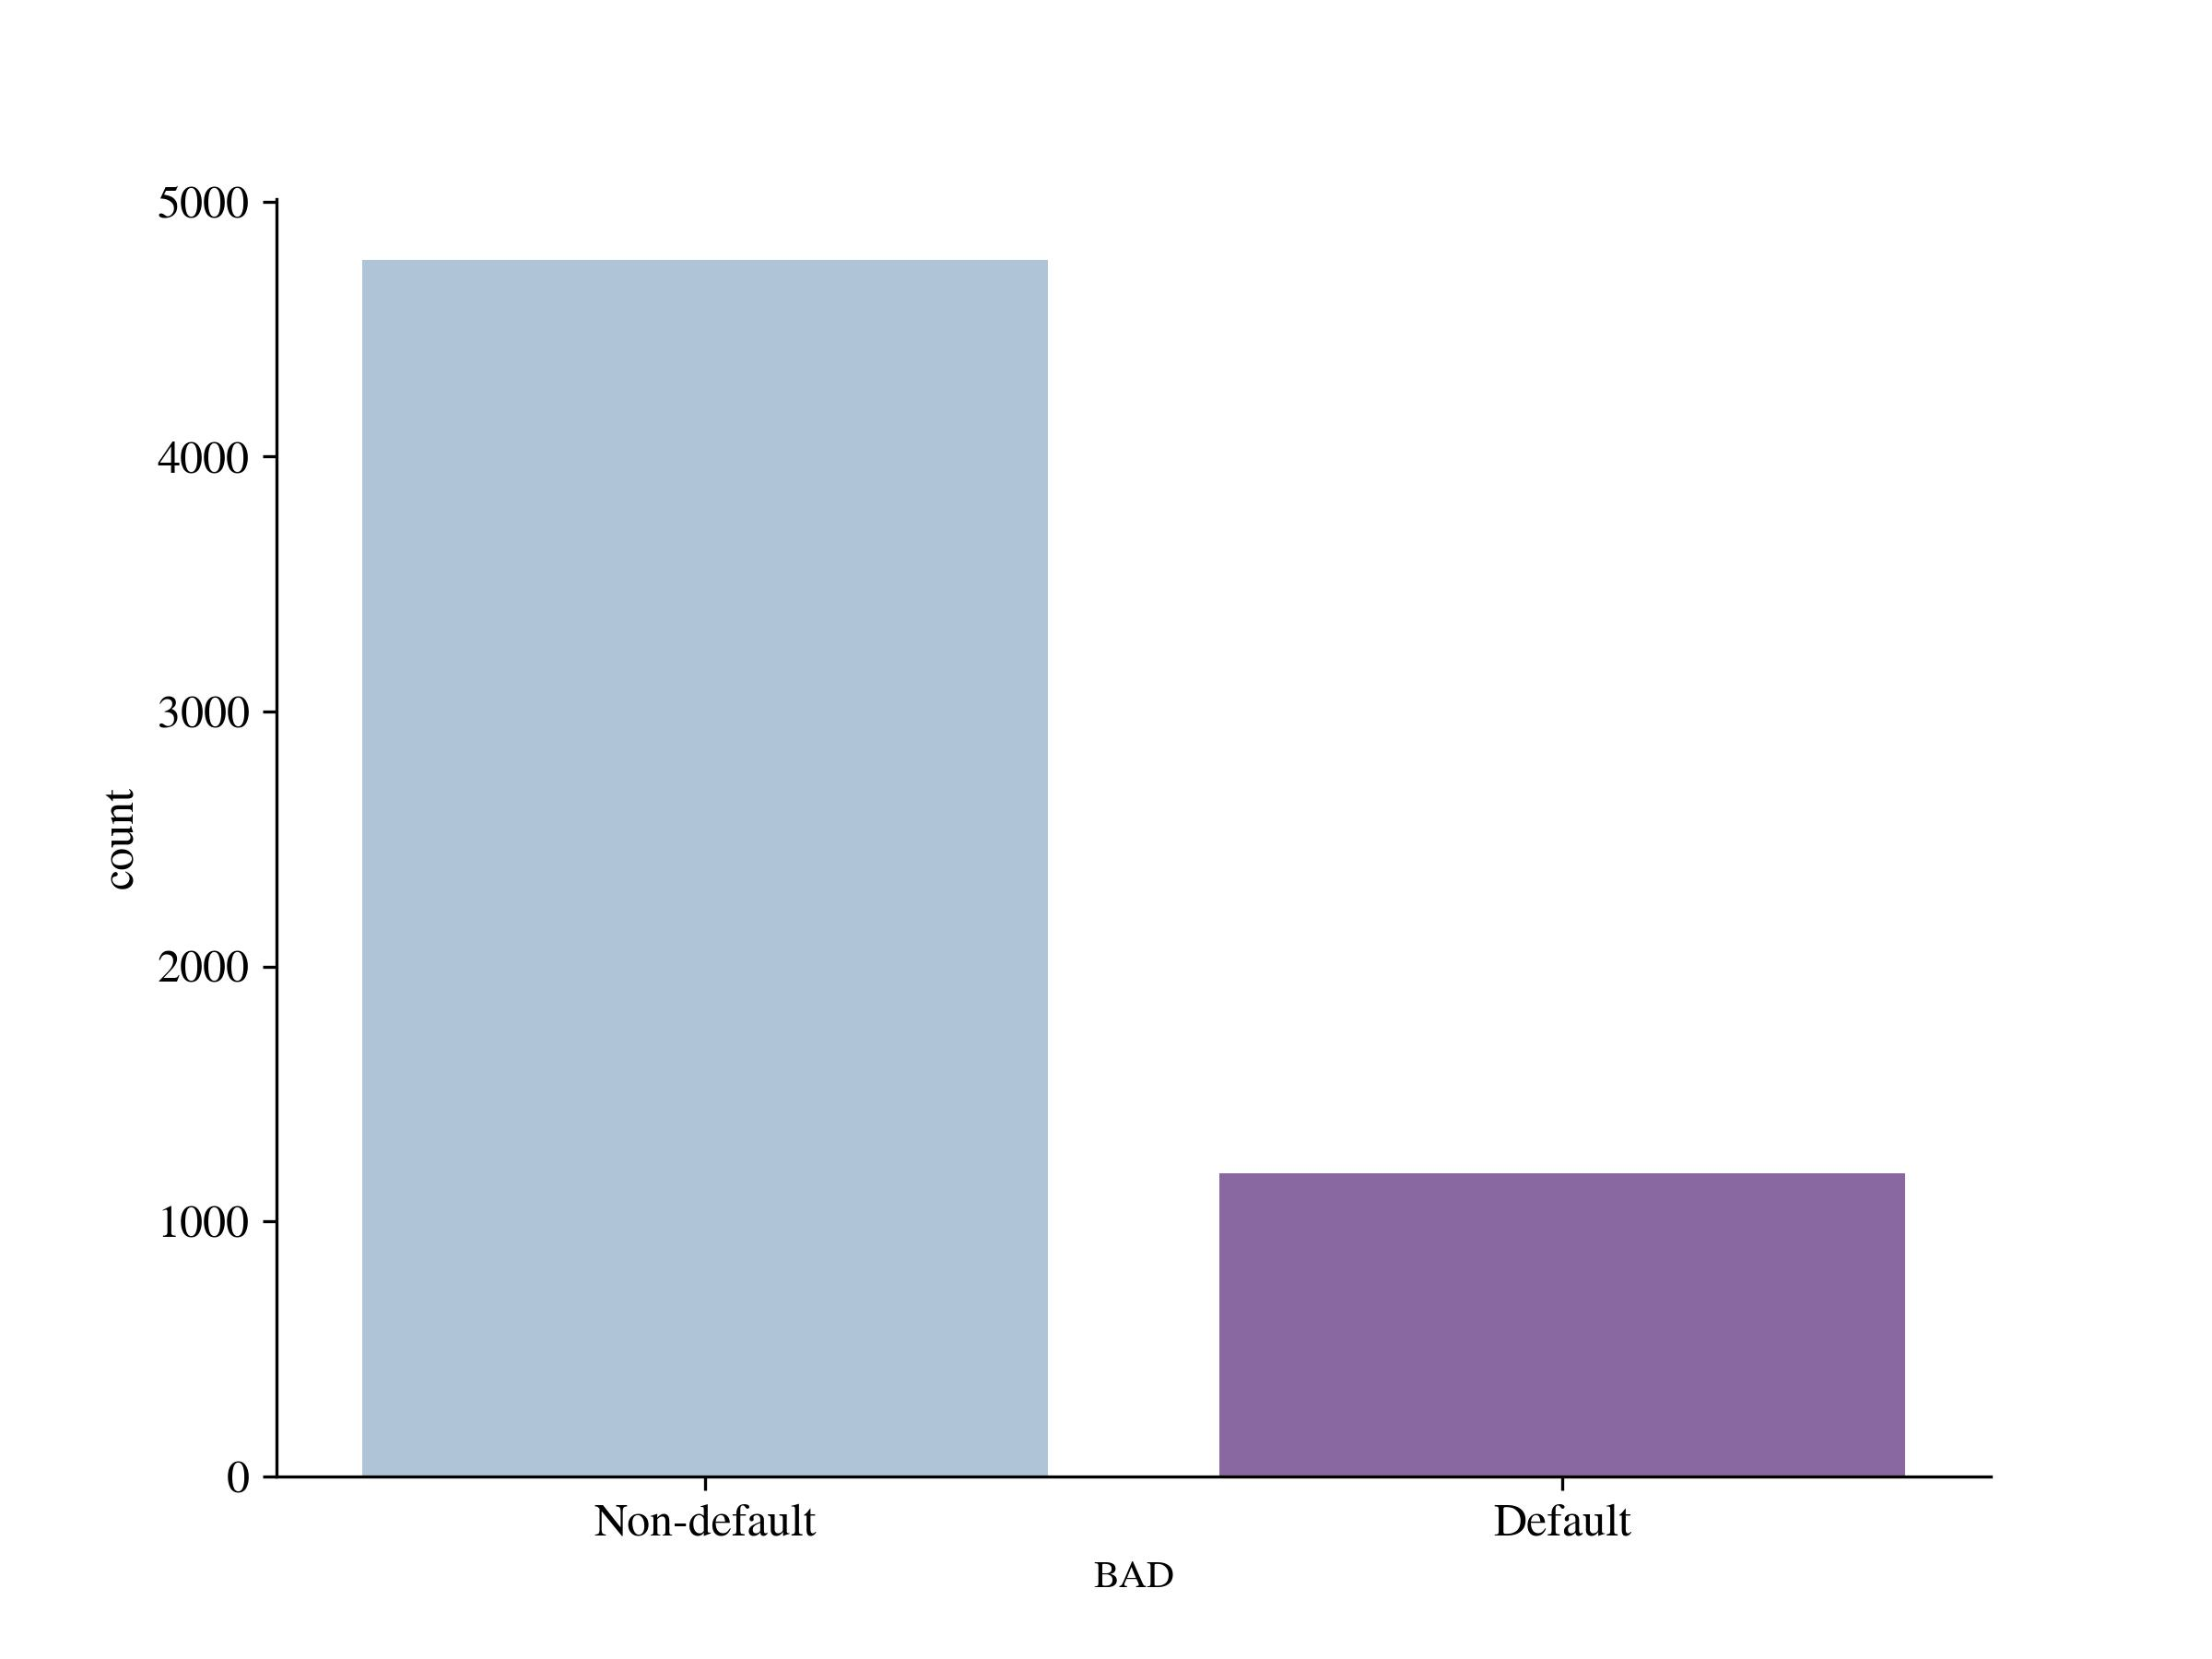
\includegraphics[width=150mm]{Figures/Default_Distribution.jpg}
\end{center}
\begin{center}
    \begin{source}Author's results in Python.\end{source}
    \end{center}
\end{figure}

\begin{figure}[H]
    \begin{center}
    \caption{Conditional distribution of numeric features -- boxplots}
    \label{fig:boxfeat}
    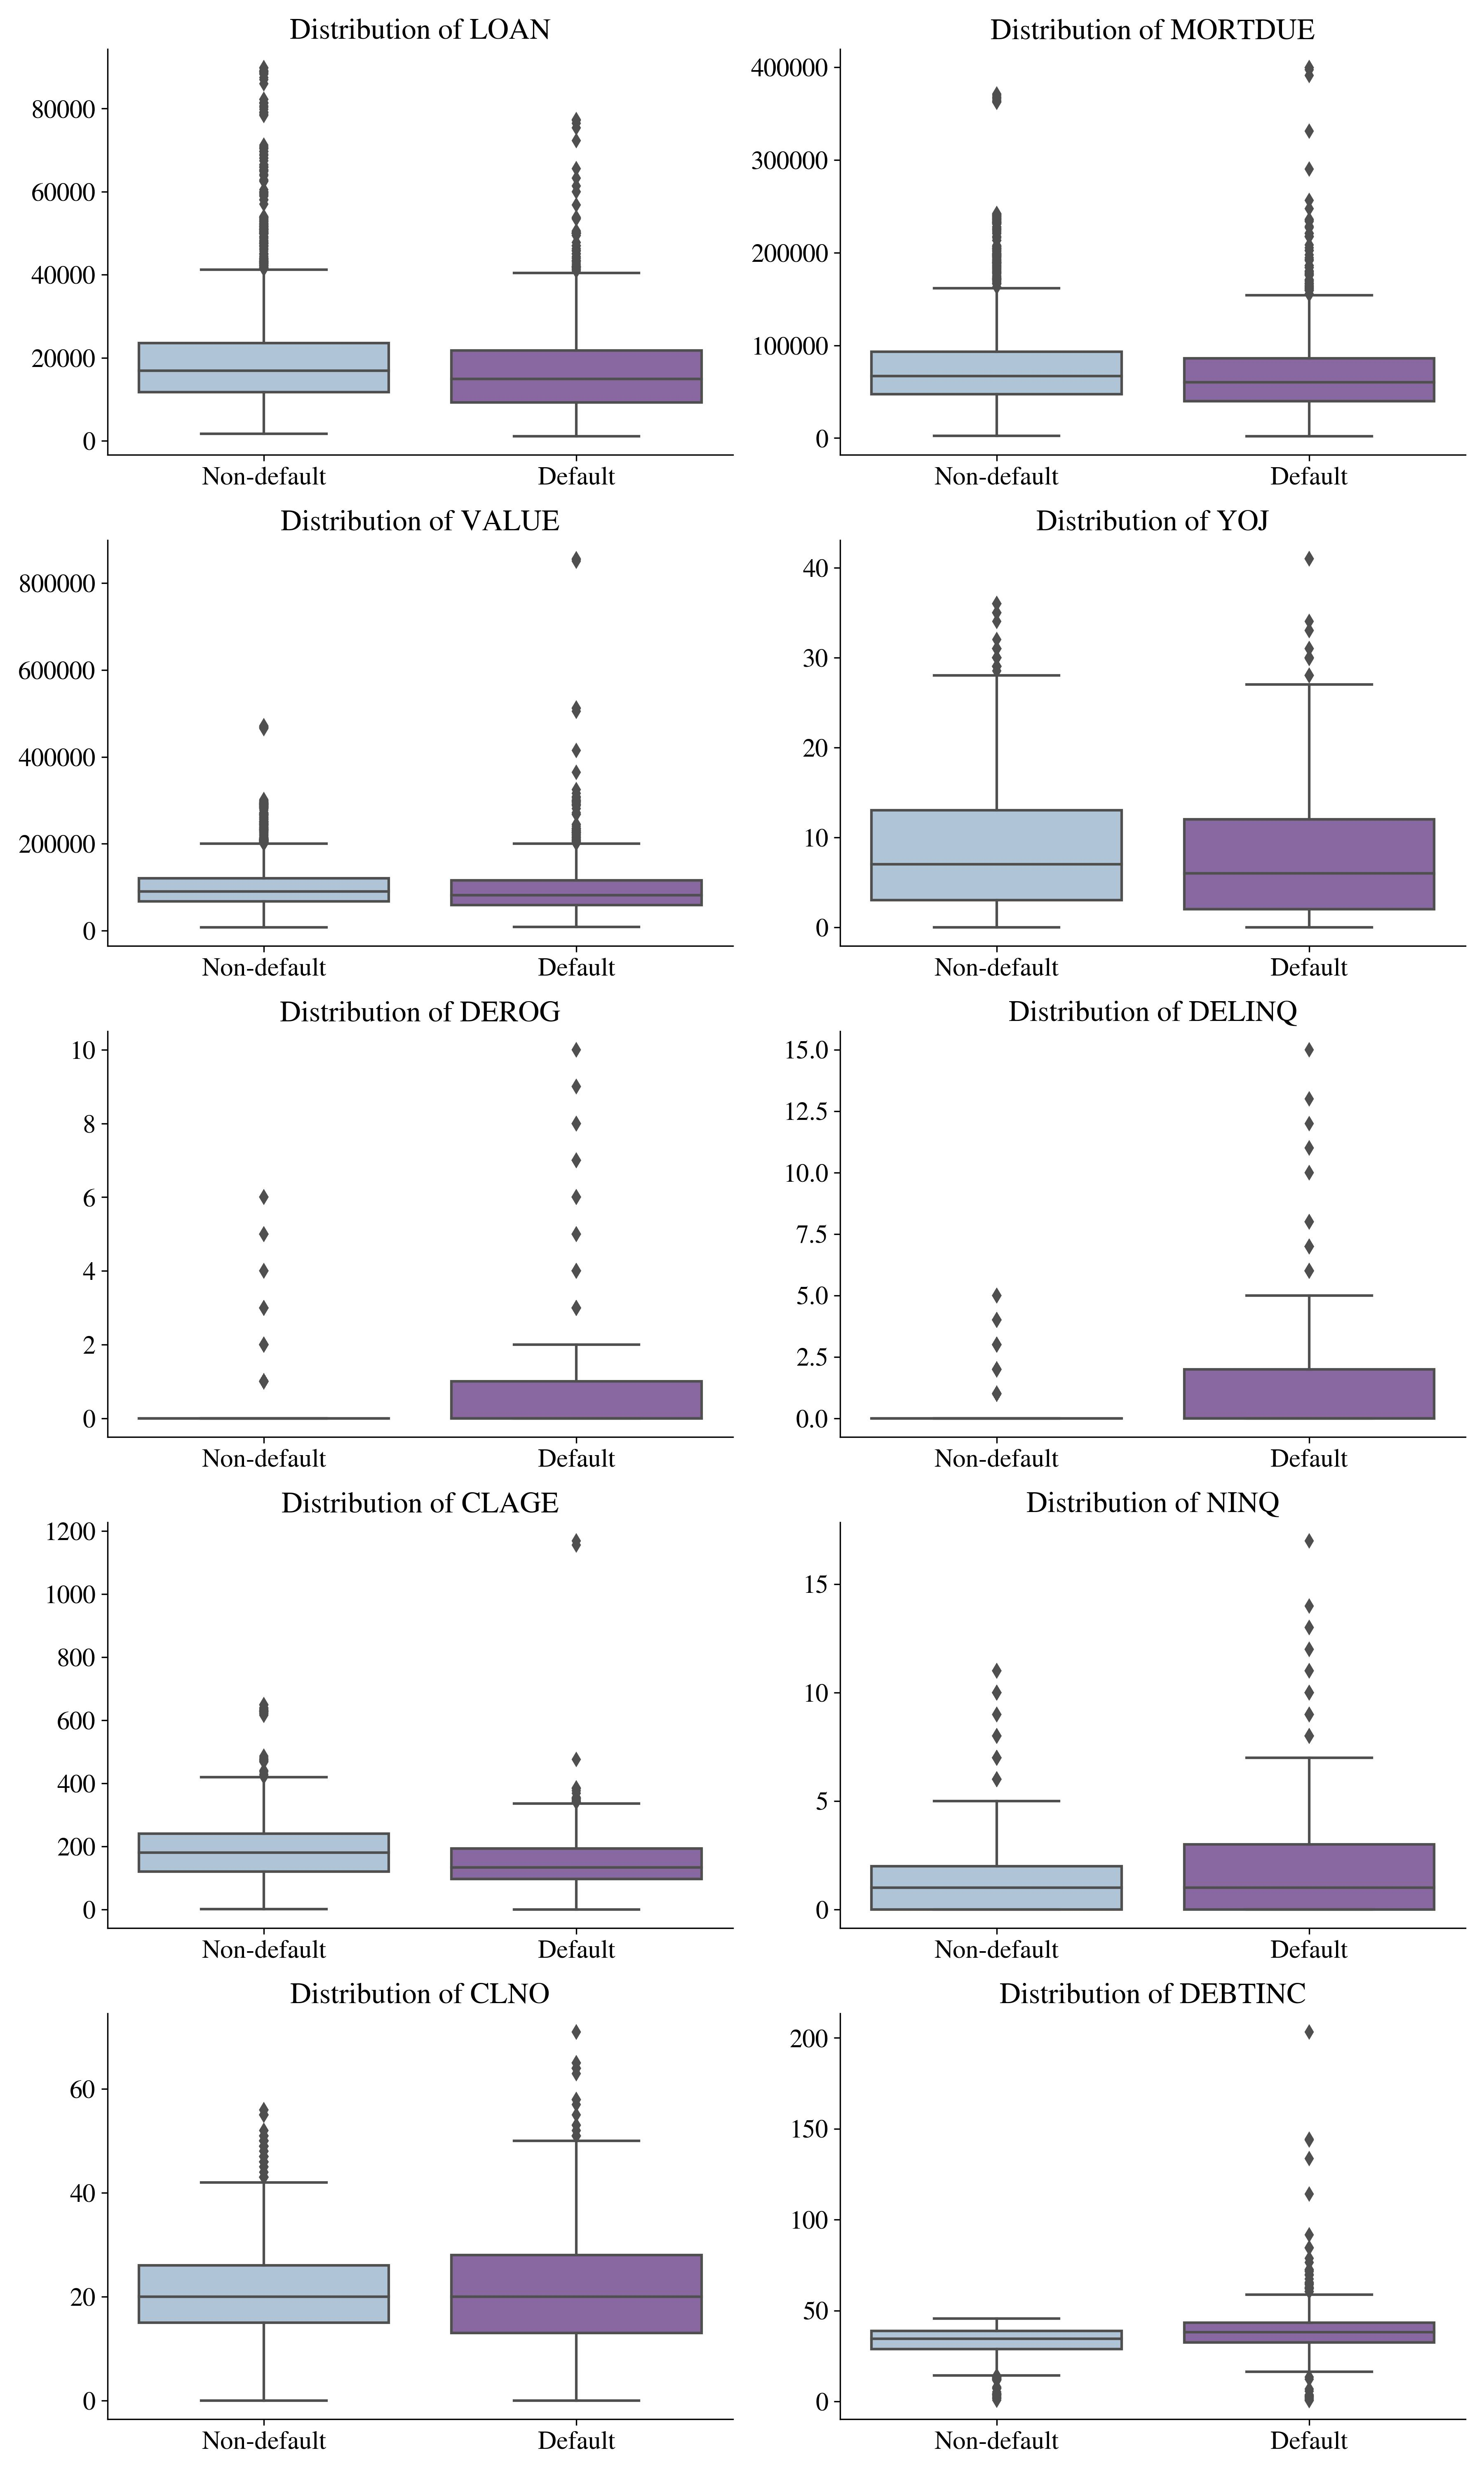
\includegraphics[width=100mm]{Figures/Continuous_Features_Distribution_Boxplots.jpg}
\end{center}
\begin{center}
    \begin{source}Author's results in Python.\end{source}
    \end{center}
\end{figure}

\begin{figure}[H]
    \begin{center}
    \caption{Conditional distribution of numeric features -- histograms}
    \label{fig:histfeat}
    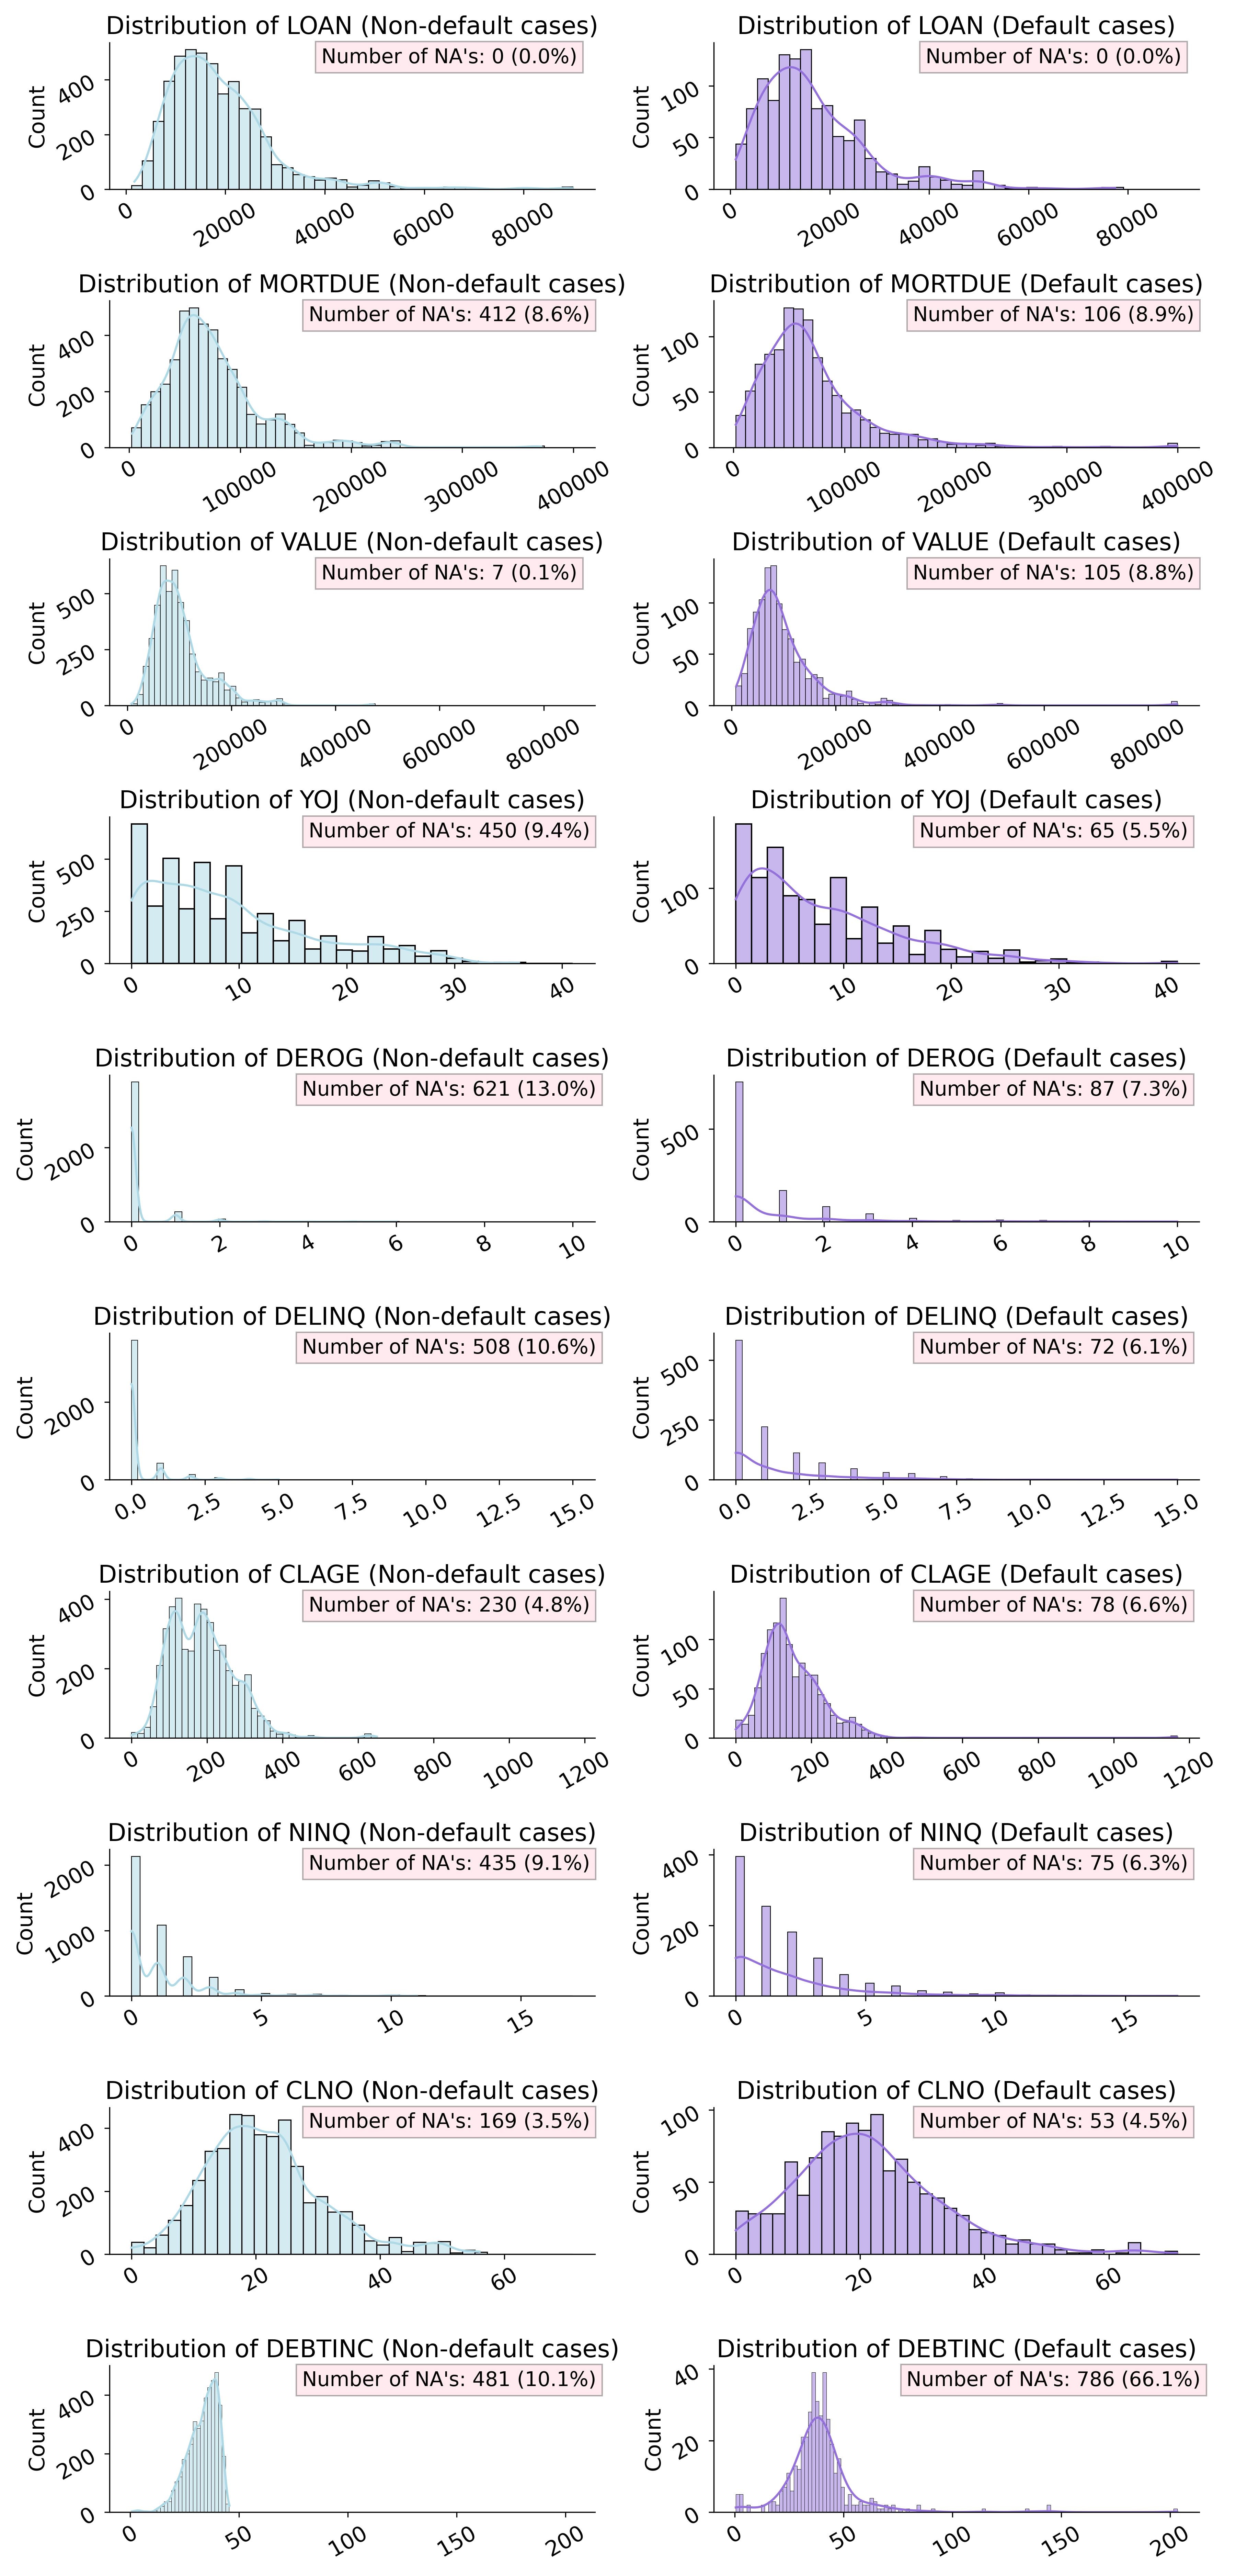
\includegraphics[width=110mm]{Figures/Continuous_Features_Distribution_Histograms.jpg}
\end{center}
\begin{center}
    \begin{source}Author's results in Python.\end{source}
    \end{center}
\end{figure}

\begin{figure}[H]
    \begin{center}
    \caption{Conditional distribution of categorical features}
    \label{fig:catdist}
    \includegraphics[width=100mm]{Figures/Categorical_Features_Distribution.jpg}
\end{center}
\begin{center}
    \begin{source}Author's results in Python.\end{source}
    \end{center}
\end{figure}

\subsection{Association Analysis}
In this subsection, we focus on the association analysis in order to inspect potential relationships between the variables. First, we inspect the association between the default status and the features and aftewards, we check for the association amongst the features themselves.
\subsubsection{Target Association}

In order to measure an association between the target variable and the numeric features, we use Point--Biserial correlation which denotes the value of Pearson's product moment correlation between the continuous variable and dichotomous variable \citep{kornbrot2014point}. Such coefficient ranges from -1 to +1.

\begin{equation}\label{eq}
    r_{pb,X} =  \frac{\mu \left( X | Y=1 \right) -\mu \left( X | Y=0 \right)}{\sigma_{X}}\sqrt{\frac{N\left(Y=1\right) \times N\left(Y=0\right)}{N \left(N - 1 \right)}}
\end{equation}

where $\mu \left( X | Y=1 \right)$ and $\mu \left( X | Y=0 \right)$ are the means of given numeric feature $X$ conditional on the default status and non--default status, respectively, $\sigma_{X}$ is the standard deviation of given numeric feature $X$, $N\left(Y=1\right)$ and $N\left(Y=0\right)$ are the numbers of observations with default status and non--default status, respectively, and $N$ is the total number of observation within given feature $X$.



In the following \autoref{tab:pointbi}, we can observe the computed Point-Biserial coefficient for each numeric feature with respect to the default status, including its statistical significance. As can be seen, features such as \texttt{DEROG}, \texttt{DELINQ} and \texttt{DEBTINC} are moderately and positively association with default status on 1\% statistical significance level. Thus, we can infer that these features could be important predictors within modelling based on such association analysis.

    \begin{table}[H]
        \small
        \setlength{\tabcolsep}{8pt}
        \renewcommand{\arraystretch}{1.3}
        \begin{center}
            \caption[Dataset columns]{Point--Biserial Correlation table}\label{tab:pointbi}
            \begin{tabular}{@{} l r @{\hspace{1cm}} l @{}}
        \toprule
        \textbf{Feature} & \textbf{Coefficient} & \textbf{Significance}\\
        \midrule
        \hline
        LOAN & -0.075  & ***\\
        \hline
        MORTDUE & -0.048  & ***\\
        \hline
        VALUE & -0.030  & ** \\
        \hline
        YOJ & -0.060  & *** \\
        \hline
        DEROG & 0.276 & *** \\
        \hline
        DELINQ & 0.354 & *** \\
        \hline
        CLAGE & -0.170 & *** \\
        \hline
        NINQ & 0.175 & *** \\
        \hline
        CLNO & -0.004 & \\
        \hline
        DEBTINC & 0.200 & *** \\
        \bottomrule
        \end{tabular}
        \end{center}

        \begin{center} % Center the source
    
            \footnotesize{$^{*}$: $p<0.10$, $^{**}$: $p<0.05$, $^{***}$: $p<0.01$}

        \end{center}
            \begin{center}

            \source{Author's results in Python}
        \end{center}
    \end{table}

For measuring a relationship's strength between the dichotomous and categorical variables

\begin{equation}\label{eq}
		CV_{X} = \sqrt{\frac{\chi^{2}}{N\left(k-1\right)}}
		\end{equation}

        \begin{table}[H]
            \small
            \setlength{\tabcolsep}{8pt}
            \renewcommand{\arraystretch}{1.3}
            \begin{center}
                \caption[Dataset columns]{Cramer's V Association table}\label{tab:values}
                \begin{tabular}{@{} l r @{\hspace{1cm}} l @{}}
            \toprule
            \textbf{Feature} & \textbf{Coefficient} & \textbf{Significance}\\
            \midrule
            \hline
            JOB & 0.120  & ***\\
            \hline
            REASON & 0.038  & ***\\
            \bottomrule
        \end{tabular}
    \end{center}
    \begin{center} % Center the source
        \footnotesize{$^{*}$: $p<0.10$, $^{**}$: $p<0.05$, $^{***}$: $p<0.01$}
    \end{center}
        \begin{center}
        \source{Author's results in Python}
    \end{center}
\end{table}



Phi coefficient - association between the binary variables:


\begin{equation}\label{eq}
    \phi_{X} = \sqrt{\frac{\chi^{2}}{n}}
    \end{equation}


    \begin{table}[H]
        \small
        \setlength{\tabcolsep}{8pt}
        \renewcommand{\arraystretch}{1.3}
        \begin{center}
            \caption[Dataset columns]{Phi Coefficient Correlation table}\label{tab:values}
            \begin{tabular}{@{} l r @{\hspace{1cm}} l @{}}
        \toprule
        \textbf{Feature} & \textbf{Coefficient} & \textbf{Significance}\\
        \midrule
        \hline
        LOAN & 0.000  & \\
        \hline
        MORTDUE & 0.003  & \\
        \hline
        VALUE & 0.254  & *** \\
        \hline
        REASON & 0.004 & \\
        \hline
        JOB & 0.064 & *** \\
        \hline
        YOJ & 0.056  & *** \\
        \hline
        DEROG & 0.070 & *** \\
        \hline
        DELINQ & 0.061 & *** \\
        \hline
        CLAGE & 0.030 & ** \\
        \hline
        NINQ & 0.039 & *** \\
        \hline
        CLNO & 0.018 & \\
        \hline
        DEBTINC & 0.547 & *** \\
        \bottomrule
        \end{tabular}
        \end{center}

        \begin{center} % Center the source
    
            \footnotesize{$^{*}$: $p<0.10$, $^{**}$: $p<0.05$, $^{***}$: $p<0.01$}

        \end{center}
            \begin{center}

            \source{Author's results in Python}
        \end{center}
    \end{table}

\subsubsection{Features Association}

\begin{equation}\label{eq}
	\rho_{spearman} = 1 - \frac{6 \sum_{i=1}^{n} d_{i}^{2}}{n \left(n^{2}-1\right)}
	\end{equation}

    \begin{figure}[H]
        \begin{center}
        \caption{Spearman Correlation Matrix}
        \label{fig:supply}
        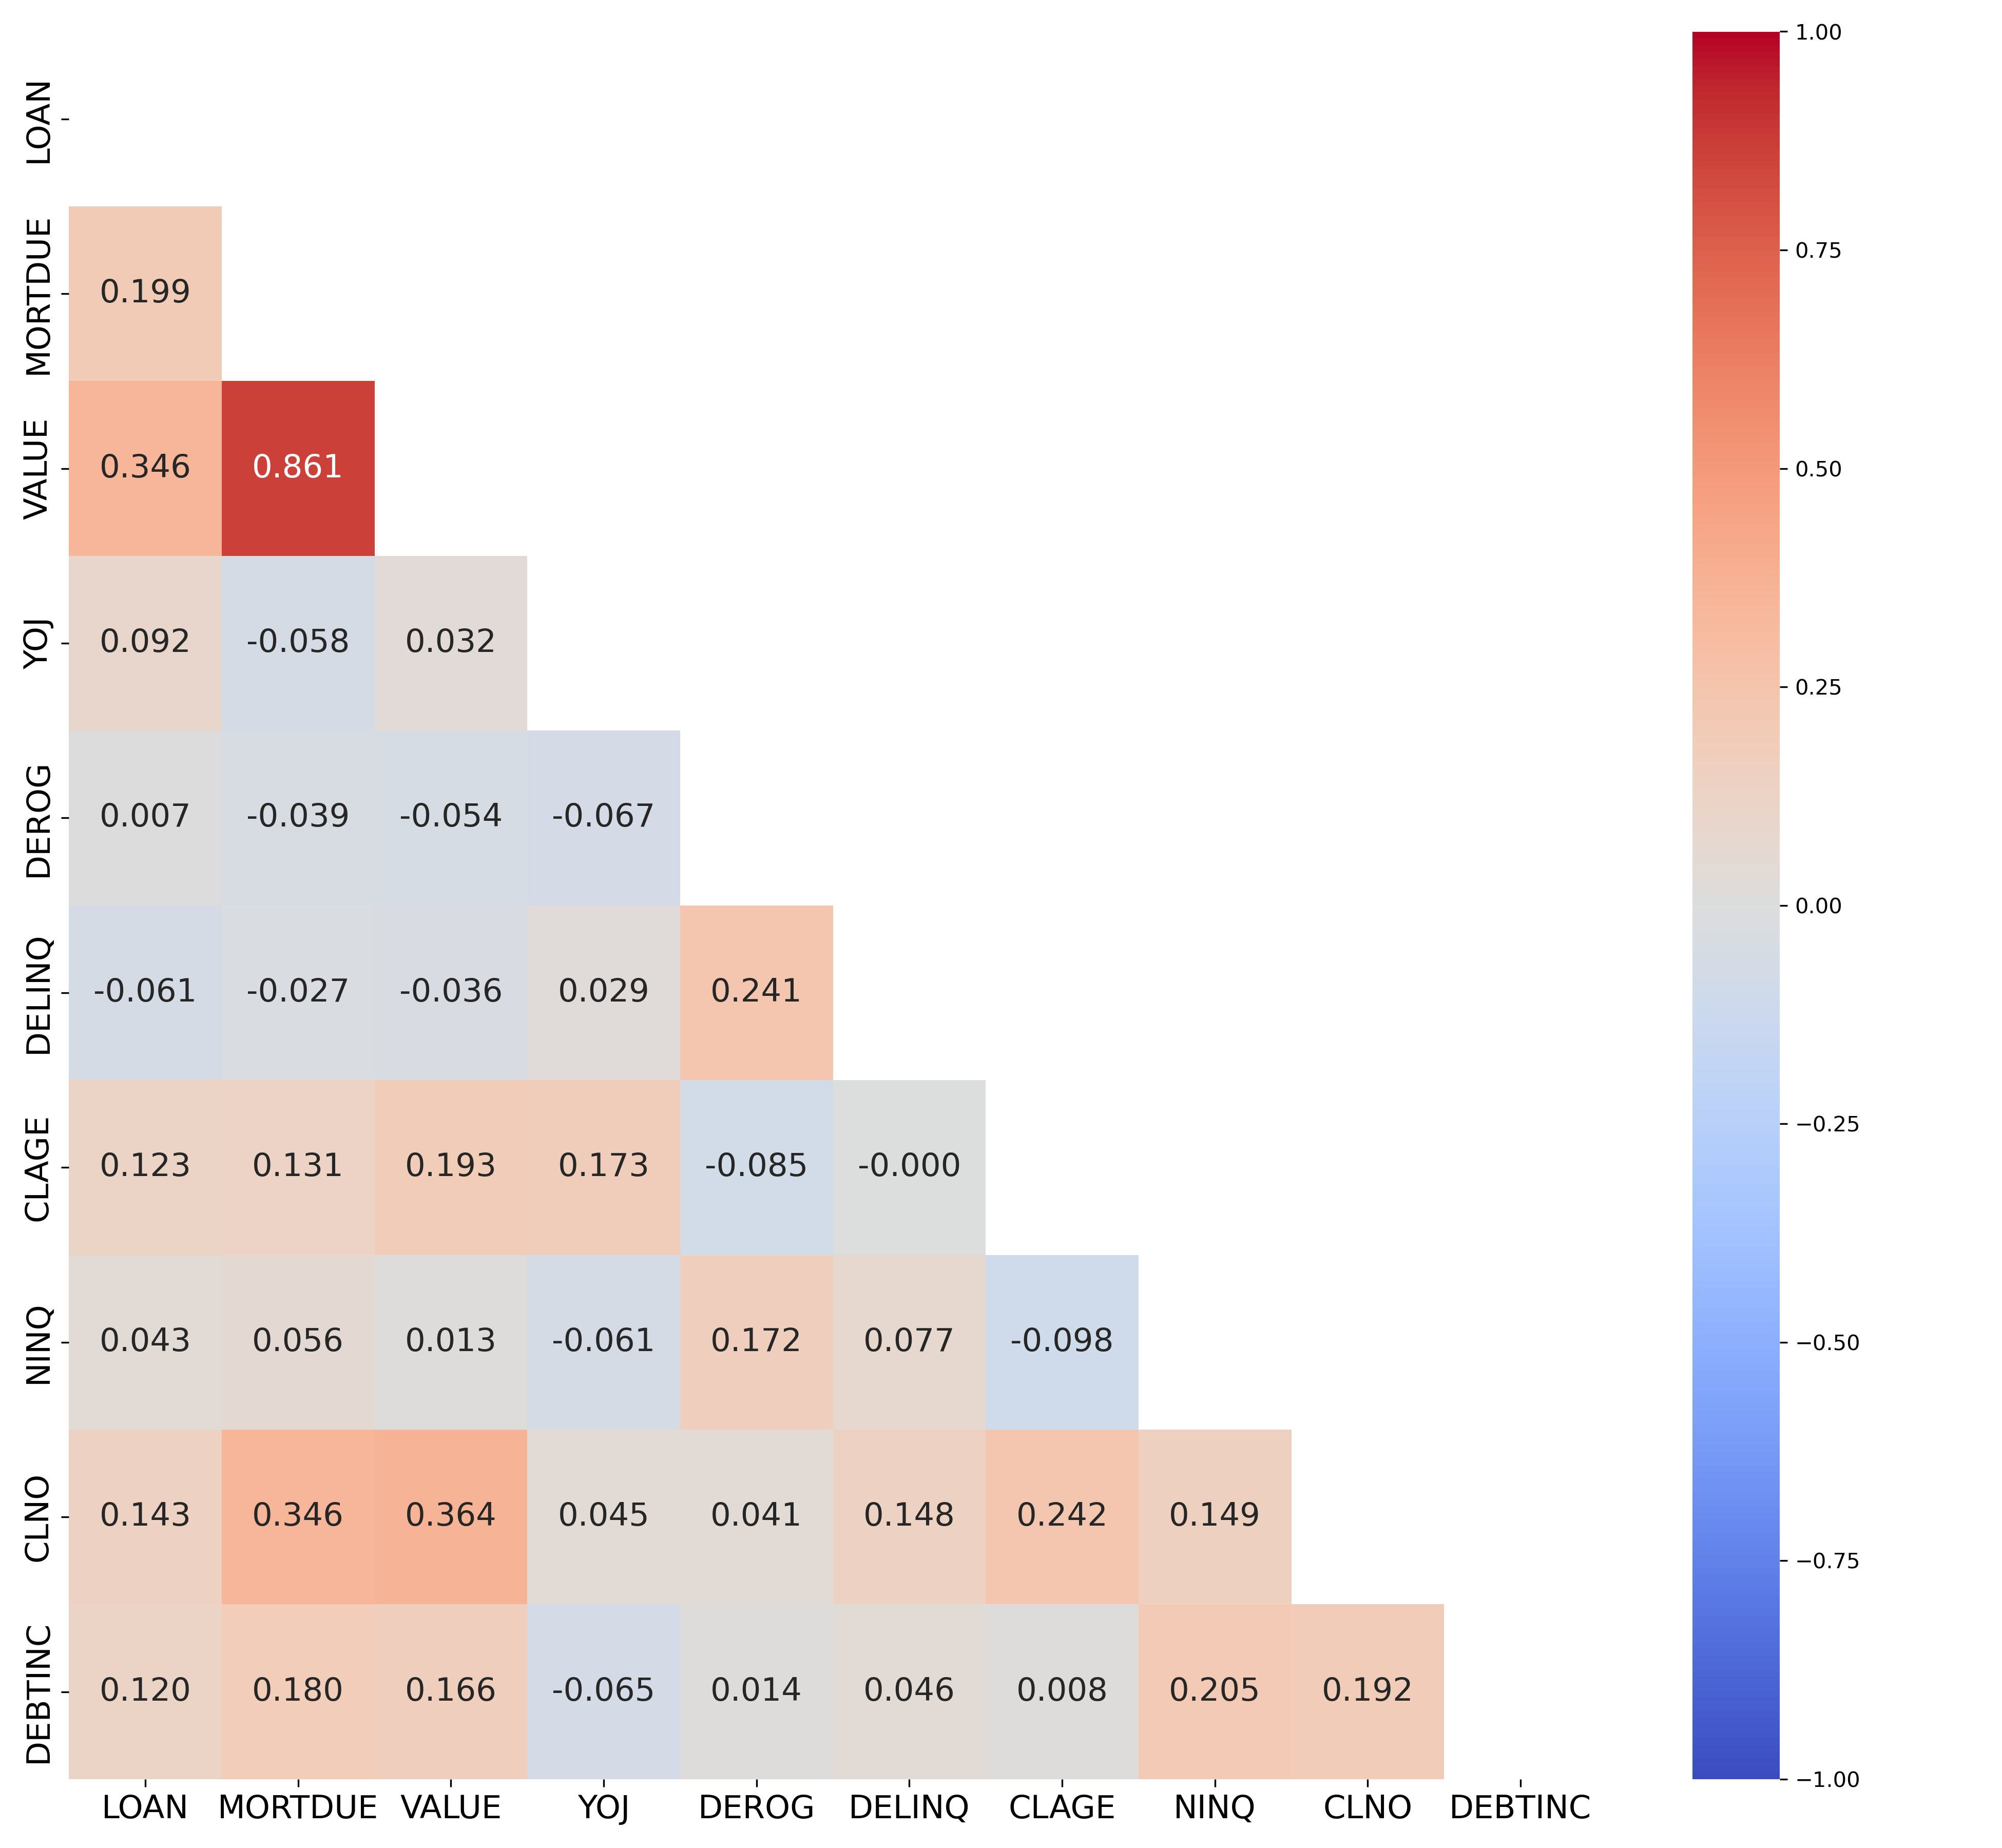
\includegraphics[width=150mm]{Figures/Spearman_Correlation_Matrix_Continuous_Features.jpg}
    \end{center}
    \begin{center}
        \begin{source}Author's results in Python.\end{source}
        \end{center}
    \end{figure}


    \begin{figure}[H]
        \begin{center}
        \caption{Nullity dendrogram}
        \label{fig:supply}
        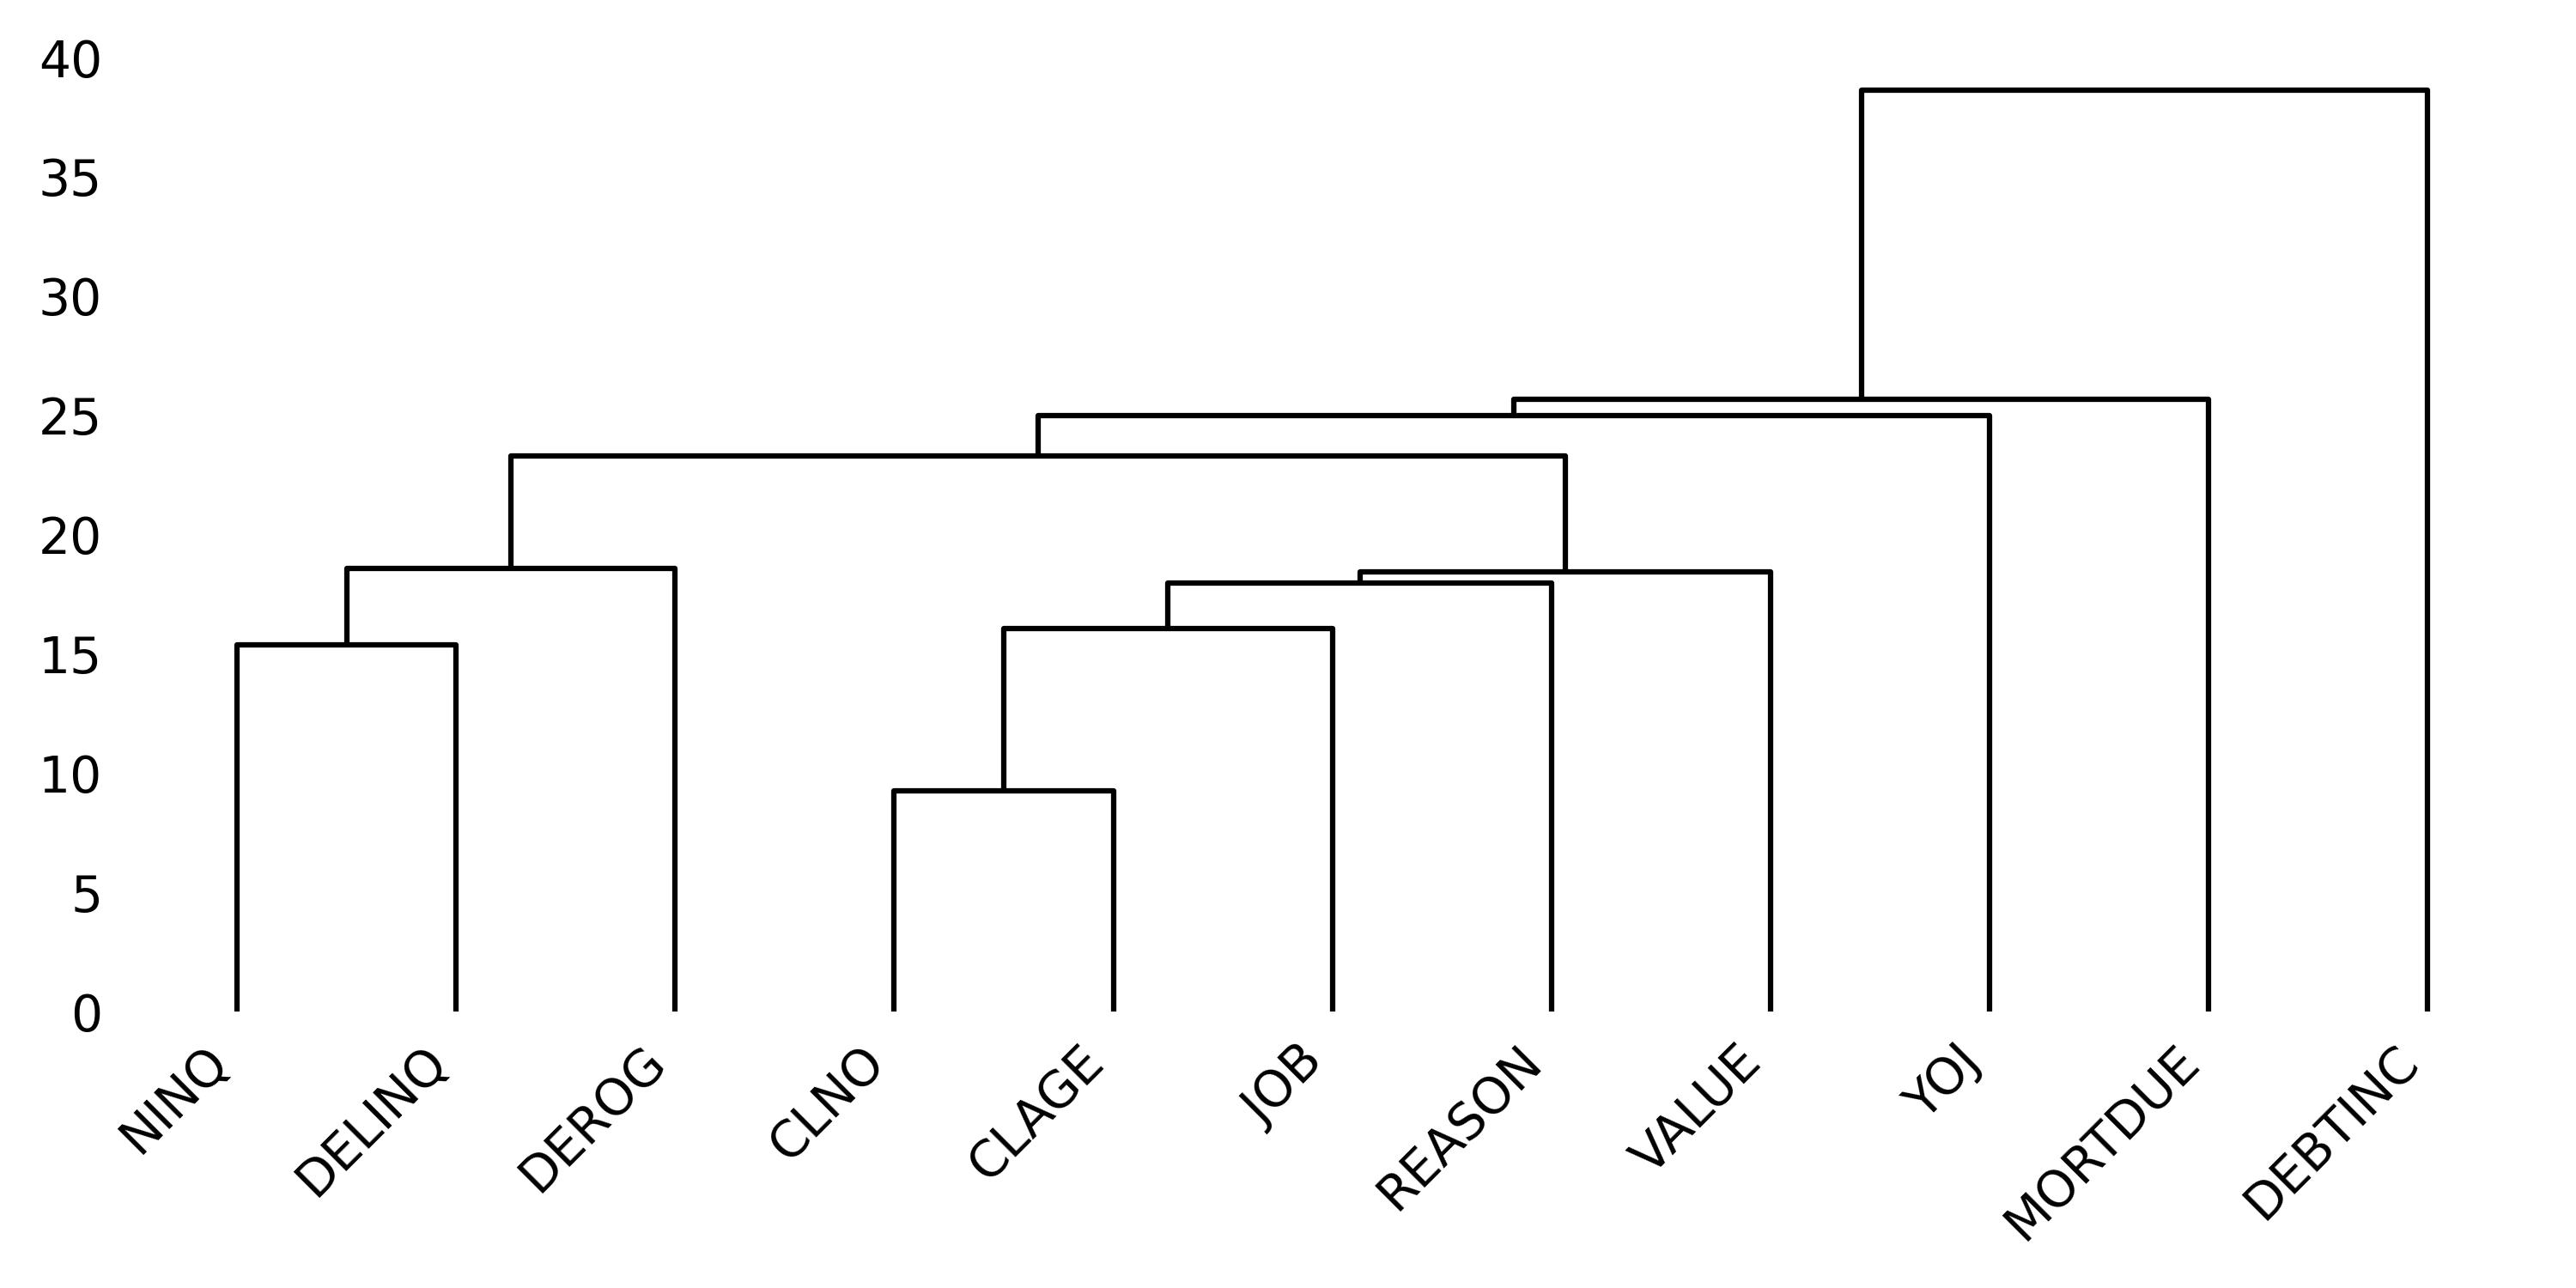
\includegraphics[width=150mm]{Figures/NA_Dendrogram.jpg}
    \end{center}
    \begin{center}
        \begin{source}Author's results in Python.\end{source}
        \end{center}
    \end{figure}
    

    \begin{figure}[H]
        \begin{center}
        \caption{Phi Correlation Matrix}
        \label{fig:supply}
        \includegraphics[width=150mm]{Figures/Phi_Correlation_NA_Features.jpg}
    \end{center}
    \begin{center}
        \begin{source}Author's results in Python.\end{source}
        \end{center}
    \end{figure}


\section{Data Preprocessing}
\subsection{Data Split and ADASYN Oversampling}
\subsection{Optimal Binning and WoE Encoding}
\section{Modelling}
\subsection{Feature Selection}
\subsection{Model Selection}
\subsection{Model Building}
\section{Model Evaluation}
\subsection{Confusion Matrix}
\subsection{Metrics Scores}
\subsection{ROC Curve}
\subsection{Learning Curve}
\subsection{SHAP Values}
\section{Machine Learning Deployment}
\subsection{Final Model Building}
\subsection{Web Application}

\section{Itemization and Environments}

Many people use simple n-dash in many occasions -- like this --, where however typographic convention---it looks a bit strange at first sight---requires m-dash.
Text text text text text text \citet{Haufler2006}. 

Text text text text text text text text text text. Text text text text text text \citet{Wells2001}. Let us describe the following animals:

\begin{description}
\item[Item 1] Text text text text text text text text text text text text text text text.
\item[Item 2] Text text text text text text text text text text text text text text text.
\end{description}

See what Edmund Burke said about the duties of a Member of Parliament (Speech To The Electors Of Bristol At The Conclusion Of The Poll, November 3, 1774):

\begin{quotesmall}
It ought to be the happiness and glory of a representative to live in the strictest union, the closest correspondence, and the most unreserved communication with his constituents. 
Their wishes ought to have great weight with him; their opinion, high respect; their business, unremitted attention.
It is his duty to sacrifice his repose, his pleasures, his satisfactions, to theirs; and above all, ever, and in all cases, to prefer their interest to his own.
But his unbiased opinion, his mature judgment, his enlightened conscience, he ought not to sacrifice to you, to any man, or to any set of men living.
These he does not derive from your pleasure; no, nor from the law and the constitution.
They are a trust from Providence, for the abuse of which he is deeply answerable.
Your representative owes you, not his industry only, but his judgment; and he betrays, instead of serving you, if he sacrifices it to your opinion.
\end{quotesmall}

Text text text text text text text text text text text text text text text.

\begin{listi}
	\item The first item, the first item, the first item, the first item, the first item, the first item,
	\item and the second item.
\end{listi}

\begin{lista}
	\item The first item, the first item, the first item, the first item, the first item, the first item, 
	\item and the second item.
\end{lista}

TText text text text text text \citet{Blomstrom2003}. 